\documentclass[11pt,a4paper]{article}
\usepackage[T1]{fontenc}
\usepackage[utf8]{inputenc}
\usepackage{mathpazo}
\usepackage{microtype}
\usepackage[a4paper,margin=23mm]{geometry}
\usepackage{amsmath,amssymb,amsthm,mathtools,mathrsfs}
\usepackage{booktabs,tabularx,array}
\usepackage{tikz,pgfplots}
\usepackage{hyperref}
\pgfplotsset{compat=1.18}
\hypersetup{colorlinks=true,linkcolor=black,citecolor=black,urlcolor=blue!45!black,
  pdftitle={Proof-Carrying Diagnostics and Spectral Bounds for Four-Dimensional Wilson SU(2)},
  pdfauthor={Tony Newton}}
\setlength{\emergencystretch}{2em}
\setlength{\parindent}{1.2em}
\setlength{\parskip}{0pt}
\numberwithin{equation}{section}
\newtheorem{theorem}{Theorem}[section]
\newtheorem{proposition}[theorem]{Proposition}
\newtheorem{lemma}[theorem]{Lemma}
\newtheorem{remark}[theorem]{Remark}
\newcommand{\SU}{\operatorname{SU}(2)}
\newcommand{\E}{\mathbb E}
\newcommand{\Cov}{\operatorname{Cov}}
\newcommand{\Var}{\operatorname{Var}}
\newcommand{\Tr}{\operatorname{Tr}}
\newcommand{\Lip}{\operatorname{Lip}}
\newcommand{\dd}{\,\mathrm d}

\title{\vspace{-0.8cm}\bfseries
Proof-Carrying Diagnostics and Spectral Bounds\\
for Four-Dimensional Wilson \(\SU\)}
\author{Tony Newton}
\date{26 October 2026}

\begin{document}
\maketitle
\begin{abstract}
The Wilson lattice provides a concrete non-Abelian gauge model, but finite
simulation and finite-spacing spectral information must be distinguished
from a construction of quantum Yang--Mills theory in four dimensions.
We give a unified analysis of a periodic four-dimensional \(\SU\)
model with reproducible numerical diagnostics and exact rational
certificates. An explicit gauge-projected transfer operator connects
its positive character expansion with temporal correlators. Using a
concentration-uniform Poincar\'e inequality on the three-sphere,
chordal Wasserstein comparison, and the classical Dobrushin method,
we reconstruct a volume-uniform bound
\(\lambda_n/\lambda_0\leq 6\beta\) for the excited
gauge-invariant transfer eigenvalues when \(0<\beta<1/6\).
We separately prove an exact zero-coupling plaquette covariance and
the bias produced by sample-mean centring, give controlled character
truncation errors, and exhibit a positive-transfer counterexample
to inferring a uniform gap from finite correlators.
The verification layer replays finite rational consequences, with
analytic hypotheses and stochastic diagnostics recorded as distinct
claim classes. The strong-coupling estimate relies on established
comparison methods and does not establish a continuum mass gap.
\end{abstract}

\section{The question and the principal result}

The mass-gap problem asks for a nontrivial quantum Yang--Mills theory
on four-dimensional Euclidean space with a strictly positive excitation
threshold after its axiomatic construction \cite{JaffeWitten}.
A positive spectral estimate on a fixed lattice is a different
statement. It can nevertheless be useful when the lattice observable,
the transfer operator, and the limiting operation are specified precisely.

We use the Wilson action on a periodic four-dimensional hypercubic
lattice with link group \(G=\SU\). In our normalization
\(W(g)=\frac12\operatorname{Re}\Tr(g)\), so \(W(g)\in[-1,1]\), and the
Gibbs weight is \(\exp(\beta\sum_p W(U_p))\).
Let \(\mathcal T_\beta\) denote the actual gauge-invariant,
positive Euclidean-time transfer operator defined in Section~2,
and let \(0\leq\lambda_n\leq\lambda_0\) be its eigenvalues.
The spatial periods \(L_1,L_2,L_3\) are integers at least two;
no condition on their common size is imposed.

\begin{theorem}[Finite-spacing, gauge-invariant spectral estimate]
\label{thm:main}
For every \(0<\beta<1/6\), the maximal transfer eigenvalue
\(\lambda_0>0\) is simple, and
\begin{equation}
 0\leq \frac{\lambda_n}{\lambda_0}\leq 6\beta<1
 \quad(n\geq1),\qquad
 \Delta_{\mathrm{lat}}
 :=\inf_{n\geq1}-\log\frac{\lambda_n}{\lambda_0}
 \geq-\log(6\beta)>0.                         \label{eq:main}
\end{equation}
Here \(-\log0=+\infty\). The bound is independent of the three
spatial periods, but is expressed in \emph{lattice-time units}.
\end{theorem}

The proof in Section~4 makes explicit a useful route through
the unit-quaternion geometry of \(G\). It is a specialization of
classical reflection positivity and Gibbs comparison methods
\cite{OsterwalderSeiler,Follmer,RebeschiniVanHandel}.
A recent, unrefereed pair of papers discusses the \(1/6\)
comparison and reports a stronger range \(\beta<2/9\) using
a sharp Wasserstein estimate
\cite{BhattacharjeeBhattacharyaShort,BhattacharjeeBhattacharya};
we neither establish that sharper estimate nor claim
priority for the \(1/6\) threshold.
Our contribution is a traceable finite-model reconstruction that
places the transfer proof, exact rational enclosures, a rigorous
null model, and deliberately limited numerical evidence within
one set of verified interfaces.

\section{Wilson geometry and the physical transfer operator}
\label{sec:transfer}

Let the Euclidean torus have extents \((T,L_1,L_2,L_3)\)
with \(T\geq2\),
let \(V=L_1L_2L_3\), and associate \(U_{x,\mu}\in G\) to each
positively oriented link. A reversed link carries \(U_{x,\mu}^{-1}\).
For the positively oriented plaquette \(p=(x;\mu,\nu)\), set
\begin{equation}
 U_p=U_{x,\mu}U_{x+\hat\mu,\nu}
       U_{x+\hat\nu,\mu}^{-1}U_{x,\nu}^{-1},
 \qquad
 \dd\mu_{\beta,T}(U)
 =\frac{e^{\beta\sum_pW(U_p)}}{Z_{\beta,T}}
       \prod_{x,\mu}\dd H(U_{x,\mu}),             \label{eq:wilson}
\end{equation}
where \(H\) is normalized Haar measure. Under a site-gauge
transformation \(U_{x,\mu}\mapsto
h_xU_{x,\mu}h_{x+\hat\mu}^{-1}\), the plaquette trace and
measure are invariant.

At a fixed time, write \(U=(U_e)_{e=1}^{3V}\in G^{3V}\) for the
spatial positive links and
\begin{equation}
 B(U)=\sum_{\text{spatial }p}W(U_p),\qquad
 |B(U)|\leq3V,\qquad
 \mathscr H=L^2(G^{3V},H^{\otimes3V}).
\end{equation}
Let \(P\) be averaging over all site-gauge transformations on that
slice. It is an orthogonal projection onto the gauge-invariant
subspace \(\mathscr H_{\mathrm{inv}}\).
Define multiplication and temporal convolution on \(\mathscr H\) by
\begin{align}
 (M_\beta f)(U)&=e^{\beta B(U)/2}f(U),\nonumber\\
 (C_\beta f)(U)&=\int_{G^{3V}}
       \prod_{e=1}^{3V}e^{\beta W(U_eV_e^{-1})}
       f(V)\dd H^{\otimes3V}(V),                 \label{eq:transfer}\\
 \mathcal T_\beta&=M_\beta P C_\beta P M_\beta
      \quad\hbox{on }\mathscr H_{\mathrm{inv}}.\nonumber
\end{align}
An overall positive scalar in \(C_\beta\) has no effect on
transfer eigenvalue ratios. The gauge-averaged kernel contains
one Haar-integrated temporal group variable \(h_x\) per spatial
site and factors
\[
 e^{\beta[B(U)+B(V)]/2}
 \prod_{e=(x,y)}
 e^{\beta W(U_eh_yV_e^{-1}h_x^{-1})}.
\]
Each factor in the product is a timelike Wilson plaquette.
Multiplying slabs and integrating their common spatial links
reproduces \eqref{eq:wilson}, including the two spatial half-weights.
This is the familiar lattice transfer construction
\cite{OsterwalderSeiler}, implemented here with independent
gauge-transformation and plaquette-factorization checks.

For a bounded real gauge-invariant multiplication observable \(F\), its
periodic-time connected correlator has the trace formula
\begin{equation}
 C_{\beta,T,F}(t)=
  \frac{\Tr(\mathcal T_\beta^{T-t}F_c
                   \mathcal T_\beta^tF_c)}
       {\Tr(\mathcal T_\beta^T)},\qquad
 F_c=F-\langle F\rangle_{\beta,T}.               \label{eq:periodic}
\end{equation}
The positive-transfer structure makes \eqref{eq:periodic}
nonnegative for the equilibrium finite Gibbs measure. This does
\emph{not} force the same sign on every finite sampled and
sample-centred Monte Carlo correlator.

\section{Characters, exact enclosures and their meaning}
\label{sec:characters}

Identify \(G\) with the unit quaternions \(S^3\) and write
\(x=W(g)\in[-1,1]\). The character of the irreducible representation
of dimension \(d\) is \(U_{d-1}(x)\), the Chebyshev polynomial of the
second kind. With \(I_d\) the modified Bessel function,
\begin{equation}
 e^{\beta x}=\sum_{d=1}^{\infty}
        a_d(\beta)U_{d-1}(x),\qquad
 a_d(\beta)=\frac{2d}{\beta}I_d(\beta)>0.
                                                        \label{eq:chars}
\end{equation}
Schur orthogonality shows that the scalar convolution
eigenvalue on dimension-\(d\) matrix coefficients is
\(\gamma_d=2I_d(\beta)/\beta>0\).
Consequently \(C_\beta\), its gauge compression \(PC_\beta P\),
and the positive congruence in \eqref{eq:transfer} are
self-adjoint and nonnegative. Their rapidly decreasing
Peter--Weyl coefficients give compactness and trace class on a
finite spatial lattice. The gauge-averaged integral kernel is
strictly positive; Perron--Jentzsch therefore gives a simple
positive eigenfunction \(\phi_0\) for \(\lambda_0\).

The \emph{one-link} fundamental-to-trivial ratio is
\begin{equation}
 r_{\mathrm{fund}}(\beta)
   =\frac{\gamma_2}{\gamma_1}
   =\frac{I_2(\beta)}{I_1(\beta)}.                 \label{eq:besselratio}
\end{equation}
At \(\beta=2\), exact positive-series intervals contain
\begin{equation}
 r_{\mathrm{fund}}(2)
 =0.433127426722311758\ldots,\qquad
 -\log r_{\mathrm{fund}}(2)
 =0.836723306231588913\ldots.                   \label{eq:besselvalue}
\end{equation}
Neither number is an eigenvalue ratio of the full interacting
gauge-invariant transfer operator. Treating the second as a
four-dimensional physical gap would skip the gauge-projected
many-link dynamics.

The character expansion also admits a global finite-cutoff
certificate. Set \(h=\beta/2\), and truncate
\eqref{eq:chars} after dimension \(D\).
The Bessel series and character norm imply
\begin{equation}
 I_d(\beta)
 =\sum_{k=0}^{\infty}
     \frac{h^{2k+d}}{k!(k+d)!}
 \leq\frac{h^d}{d!}e^{h^2},\qquad
 |U_{d-1}(x)|\leq d.
\end{equation}
If \(r=h(D+2)/(D+1)^2<1\), the omitted pointwise kernel
contribution obeys, uniformly for \(x\in[-1,1]\),
\begin{equation}
 \left|\sum_{d>D}a_d(\beta)U_{d-1}(x)\right|
 \leq R_D(\beta):=
 \frac{2e^{h^2}}{\beta}
 \frac{(D+1)^2h^{D+1}}{(D+1)!}\frac1{1-r}.
                                                        \label{eq:tail}
\end{equation}
Indeed the displayed bound for each term has successive ratio
\(h(d+1)/d^2\), which decreases for \(d\geq D+1\);
the geometric tail begins at the \(d=D+1\) term.
In the accompanying exact implementation, Bessel sums are
enclosed by positive rational intervals and the exponential
in \eqref{eq:tail} by an outward rational Taylor estimate.
This certifies truncated kernels, not a continuum field theory.

\section{A volume-uniform lattice spectral window}
\label{sec:gap}

The essential improvement over an elementary total-variation
comparison comes from measuring a change of a single link in the
\emph{chordal} metric
\(\rho(x,y)=|x-y|\) on \(S^3\subset\mathbb R^4\).
For \(b\in\mathbb R^4\), let
\begin{equation}
 \dd\nu_b(x)=\frac{e^{b\cdot x}}{\int_{S^3}e^{b\cdot z}
       \dd\sigma(z)}\,\dd\sigma(x),             \label{eq:vmf}
\end{equation}
where \(\sigma\) is normalized spherical measure.
These are the von Mises--Fisher conditional distributions of the
Wilson links.

\begin{lemma}[Uniform spherical Poincar\'e inequality]
\label{lem:poincare}
For every \(b\in\mathbb R^4\) and smooth real
\(f:S^3\to\mathbb R\),
\begin{equation}
 \Var_{\nu_b}(f)\leq\frac13
        \int_{S^3}|\nabla_{S^3}f|^2\dd\nu_b.
                                                        \label{eq:poincare}
\end{equation}
\end{lemma}
\begin{proof}
By rotation, take \(b=\kappa e_1\) with \(\kappa\geq0\), and use
polar angle \(\theta\) from \(e_1\). The angular weight is
\(w(\theta)=\sin^2\theta\,e^{\kappa\cos\theta}\).
Expansion into degree-\(\ell\) harmonics on the residual \(S^2\)
gives the one-dimensional generator
\[
 L_\ell=\frac1w\partial_\theta(w\partial_\theta)
          -\frac{\ell(\ell+1)}{\sin^2\theta}.
\]
The constant mode at \(\ell=0\) has eigenvalue zero.
For \(\ell\geq1\) the centrifugal term increases with \(\ell\).
Writing \(\psi=\sin\theta\,e^{a\kappa\cos\theta}\),
direct differentiation yields
\begin{equation}
 -\frac{L_1\psi}{\psi}
 =3+(5a+1)\kappa\cos\theta
   -a(a+1)\kappa^2\sin^2\theta.
                                                        \label{eq:barta1}
\end{equation}
At \(a=-1/5\) this is
\(3+\frac4{25}\kappa^2\sin^2\theta\geq3\).
The positive supersolution identity
\[
 \int \bigl(|u'|^2+\ell(\ell+1)
               \csc^2\theta\,u^2\bigr)w
 =\int\psi^2|(u/\psi)'|^2w
   +\int(-L_\ell\psi)\psi(u/\psi)^2w
\]
then places every \(\ell\geq1\) eigenvalue above \(3\).
Regular modes vanish as \(O(\theta^\ell)\) at a pole; the
boundary terms vanish as \(O(\theta^{2\ell+1})\).

For a nonconstant zonal eigenfunction \(g\), write
\(L_0g=-\lambda g\), \(u=g'\), and
\(d(\theta)=2\cot\theta-\kappa\sin\theta\).
Differentiation yields
\[
 \mathcal M u=-\lambda u,\qquad
 \mathcal M=\frac1w\partial_\theta(w\partial_\theta)+d'(\theta).
\]
In this case
\begin{equation}
 -\frac{\mathcal M\psi}{\psi}
 =3+(5a+2)\kappa\cos\theta
   -a(a+1)\kappa^2\sin^2\theta.
                                                        \label{eq:barta0}
\end{equation}
With \(a=-2/5\), it is at least
\(3+\frac6{25}\kappa^2\sin^2\theta\).
The smooth zonal derivative vanishes as \(O(\theta)\) at
each pole, and its ground-state boundary term is \(O(\theta^3)\).
Thus its eigenvalue is at least \(3\).
All nonconstant spherical sectors have spectral value
at least \(3\), establishing \eqref{eq:poincare}.
\end{proof}

\begin{lemma}[Chordal conditional influence]
\label{lem:W1}
For all \(b,b'\in\mathbb R^4\),
\begin{equation}
 W_{1,\rho}(\nu_b,\nu_{b'})
          \leq\frac13|b-b'|.
                                                        \label{eq:w1}
\end{equation}
\end{lemma}
\begin{proof}
If \(f\) is one-Lipschitz in the chordal metric, its
intrinsic spherical gradient has norm at most one almost
everywhere. The same holds for \(x\mapsto h\cdot x\)
when \(|h|=1\). Cauchy--Schwarz and
\eqref{eq:poincare} give
\(|\Cov_{\nu_b}(f,h\cdot x)|\leq1/3\).
Differentiating the expectation of \(f\) along the linear
parameter path \(b_s=b+s(b'-b)\) yields
\[
 \frac{\dd}{\dd s}\E_{\nu_{b_s}}f
      =\Cov_{\nu_{b_s}}(f,(b'-b)\cdot x).
\]
Integrate over \(s\in[0,1]\) and take the supremum
over chordal one-Lipschitz \(f\) by Kantorovich duality.
\end{proof}

\begin{proposition}[Necessary constant at the Haar point]
\label{prop:quarter}
Any constant \(K\) satisfying
\(W_{1,\rho}(\nu_b,\nu_{b'})\leq K|b-b'|\)
for all \(b,b'\in\mathbb R^4\) must obey \(K\geq1/4\).
\end{proposition}
\begin{proof}
For a unit vector \(h\in\mathbb R^4\), the function
\(f(x)=h\cdot x\) is chordal one-Lipschitz.
At the Haar point \(b=0\), rotational symmetry
gives \(\E_{\nu_0}f=0\) and
\(\Var_{\nu_0}(f)=1/4\). Differentiating the
tilted expectation at \(\varepsilon=0\) yields
\[
 \left.\frac{\dd}{\dd\varepsilon}
     \E_{\nu_{\varepsilon h}}f
       \right|_{\varepsilon=0}
      =\Var_{\nu_0}(f)=\frac14.
\]
Kantorovich duality implies
\(W_{1,\rho}(\nu_0,\nu_{\varepsilon h})
 \geq |\E_{\nu_{\varepsilon h}}f-\E_{\nu_0}f|
 =\varepsilon/4+o(\varepsilon)\) for
\(\varepsilon\downarrow0\). Divide by
\(\varepsilon\) and take the limit.
\end{proof}

Thus the available proven constant \(1/3\) and the best
possible global constant \(K_\ast\) satisfy
\(1/4\leq K_\ast\leq1/3\).
If the upper endpoint were independently reduced to
\(1/4\), the same \(18\)-incidence row-sum argument
would give \(q\leq(9/2)\beta\) and the formal window
\(\beta<2/9\). Proposition~\ref{prop:quarter}
is a \emph{necessary} bound on the coefficient,
not a proof of that proposed improvement.

\begin{proof}[Proof of Theorem~\ref{thm:main}]
Condition on every link except one fixed four-dimensional
positive link \(e\). The six incident Wilson plaquettes are
linear in its unit quaternion \(x_e\), so its conditional law
is \eqref{eq:vmf} with parameter
\(b_e=\beta\sum_{p\ni e}s_{p,e}\), where each \(s_{p,e}\)
is a unit-quaternion staple. Inversion and left or right
multiplication are chordal isometries. If another link \(f\)
changes by \(\rho(x_f,x'_f)\), then
\[
 |b_e-b_e'|\leq\beta\,m(e,f)\rho(x_f,x_f'),
\]
with \(m(e,f)\) the number of common plaquette incidences,
counted with multiplicity. Exactly six plaquettes meet \(e\);
each contains three other link incidences. Hence
\(\sum_fm(e,f)=18\), also on side-length-two tori.
Lemma~\ref{lem:W1} gives the metric Dobrushin matrix
\begin{equation}
 c_{ef}\leq\tfrac{\beta}{3}m(e,f),\qquad
 \max_e\sum_fc_{ef}\leq q:=6\beta<1.
                                                        \label{eq:dobrushin}
\end{equation}

Write \(C=(c_{ef})\) on the full finite set of positive links.
For a bounded Lipschitz observable \(F\), write \(\delta_eF\)
for the supremum of
\(|F(U)-F(U')|/\rho(U_e,U'_e)\) over pairs of configurations
which agree off \(e\). Let \(F,G\) both be such observables.
The metric Gibbs comparison inequality
\cite[Corollary~2.6]{RebeschiniVanHandel} implies
\begin{equation}
 |\Cov(F,G)|\leq
 \sum_{e,f}\delta_eF\,[(I-C)^{-1}]_{ef}\,\delta_fG.
                                                        \label{eq:cov}
\end{equation}
One can obtain this covariance form by comparing a Gibbs
measure with its tilt \(e^{sG}\), dividing the comparison
by \(|s|\) and taking \(s\to0\). The coordinate diameter
of the chordal sphere is two, giving a local tilt
perturbation at most \(|s|\delta_fG\).
Because \(C\) has row sum at most \(q\), paths of length
at least \(r\) have resolvent row sum at most
\(q^r/(1-q)\). A path from the support of \(F\) on
time slice zero to its translate at time \(t\) requires
at least \(r=\min(t,T-t)\) plaquette-neighbor steps.
Thus for every fixed spatial volume and Lipschitz
gauge-invariant \(F\),
\begin{equation}
 |\Cov_{\beta,T}(F_0,F_t)|
       \leq A(F,V)q^{\min(t,T-t)},             \label{eq:mix}
\end{equation}
where \(A(F,V)\) is finite and independent of temporal
period \(T\) and separation \(t\).

The Wilson transfer in Section~\ref{sec:transfer} has a
smooth, strictly positive integral kernel on the compact
spatial configuration manifold. Its nonzero eigenfunctions
are smooth, and the Perron eigenfunction
\(\phi_0\) is bounded away from zero. Gauge-invariant
functions descend to an orbit space that may have
singular strata; smoothness is understood before this
quotient. For any normalized excited real eigenfunction
\(\phi_n\), take the bounded Lipschitz observable
\(F_n=\phi_n/\phi_0\). At fixed \(t\), the
period-\(T\) transfer correlator converges as
\(T\to\infty\) to
\[
 C_{F_n}(t)=
 \sum_{k\geq1}|\langle\phi_k,F_n\phi_0\rangle|^2
         (\lambda_k/\lambda_0)^t
   =(\lambda_n/\lambda_0)^t.
\]
Here \(\langle\phi_0,F_n\phi_0\rangle=0\).
Inequality \eqref{eq:mix}, first with \(T\to\infty\)
and then with \(t\to\infty\), implies
\((\lambda_n/\lambda_0)^t\leq A(F_n,V)q^t\);
taking \(t\)th roots gives
\(\lambda_n/\lambda_0\leq q\).
The constant \(A(F_n,V)\) need not be uniform in \(V\):
it disappears in this eigenvalue-ratio limit.
The case \(\lambda_n=0\) is immediate.
\end{proof}

\begin{figure}[t]
\centering
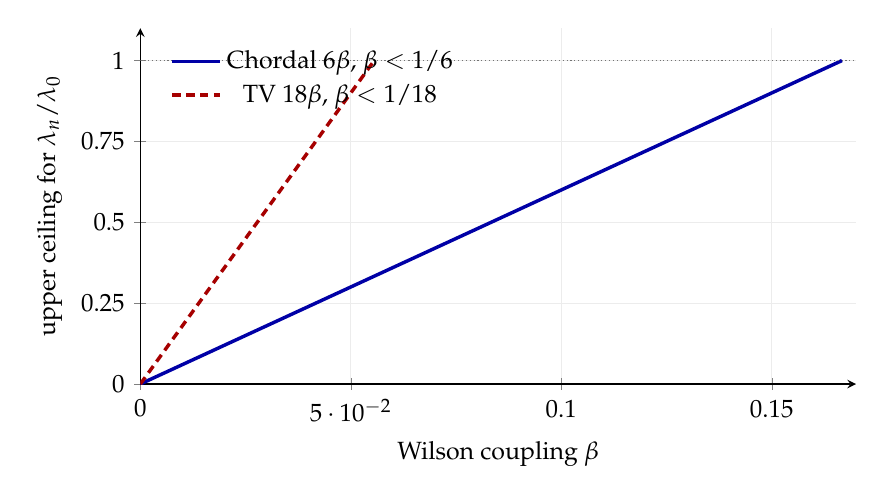
\begin{tikzpicture}
\begin{axis}[
 width=0.88\textwidth,height=6.1cm,
 xmin=0,xmax=0.17,ymin=0,ymax=1.10,
 axis lines=left,
 xlabel={Wilson coupling \(\beta\)},
 ylabel={upper ceiling for \(\lambda_n/\lambda_0\)},
 xtick={0,0.05,0.10,0.15},
 ytick={0,0.25,0.5,0.75,1.0},
 grid=major,grid style={gray!15},
 legend pos=north west,
 legend style={draw=none,fill=none,font=\small},
 every axis plot/.append style={line width=1.25pt},
 tick label style={font=\small},
 label style={font=\small},
 ]
 \addplot[blue!65!black,domain=0:0.166666,samples=80]{6*x};
 \addlegendentry{Chordal \(6\beta\), \(\beta<1/6\)}
 \addplot[red!65!black,densely dashed,domain=0:0.0555555,samples=70]{18*x};
 \addlegendentry{TV \(18\beta\), \(\beta<1/18\)}
 \addplot[black!55,thin,densely dotted,domain=0:0.17]{1};
\end{axis}
\end{tikzpicture}
\caption{Two proved small-coupling ceilings for the
gauge-invariant finite Wilson transfer spectrum. Only the portions
below one imply a positive lower gap in lattice units. The curves
are analytic bounds, not measured eigenvalues.}
\label{fig:windows}
\end{figure}

For example, \(\beta=1/10\) lies outside the elementary
total-variation range. Equations \eqref{eq:main} and
\eqref{eq:dobrushin} then give the exact bound
\begin{equation}
 \frac{\lambda_n}{\lambda_0}\leq\frac35,\qquad
 \Delta_{\mathrm{lat}}\geq-\log(3/5)
       =0.510825623765990683\ldots .           \label{eq:examplegap}
\end{equation}
Writing \(z=(1-q)/(1+q)\), the finite rational sum
\(2\sum_{j=0}^{K-1}z^{2j+1}/(2j+1)\)
is a strict lower enclosure for \(-\log q\).
Eight terms at \(q=3/5\) are retained in an exact,
tamper-checked receipt.

\section{An exact Haar null model for temporal correlators}
\label{sec:haar}

The same physical lattice gives a useful finite-sample
control at \(\beta=0\), where all positive-link variables
are independent and Haar distributed. For each time slice
define the average of its \(3V\) spatial plaquettes by
\begin{equation}
 X_t=\frac1{3V}\sum_{x\in\prod_i\mathbb Z/L_i\mathbb Z}
                 \sum_{1\leq i<j\leq3}W(U_{(t,x);ij}).
                                                        \label{eq:X}
\end{equation}
\begin{proposition}[Haar covariance and sample-mean bias]
\label{prop:haar}
For \(L_i\geq2\) and distinct time slices,
\begin{equation}
 \E_0X_t=0,\qquad
 \E_0[X_tX_u]=\frac{\mathbf1_{\{t=u\}}}{12V}.
                                                        \label{eq:haar}
\end{equation}
If \(M\) independent exact Haar-refresh configurations
are measured at all \(T\) slices, put \(N=MT\),
\(\overline X=N^{-1}\sum_{r,t}X_{r,t}\), and
\[
 \widehat C(s)=\frac1N\sum_{r,t}
 (X_{r,t}-\overline X)
 (X_{r,t+s\pmod T}-\overline X).
\]
Then, with \(v=1/(12V)\),
\begin{equation}
 \E_0\widehat C(0)=v(1-1/N),\qquad
 \E_0\widehat C(s)=-v/N\quad(1\leq s<T).
                                                        \label{eq:bias}
\end{equation}
\end{proposition}
\begin{proof}
A product of one Haar link and three fixed \(\SU\)
links is Haar. The real quaternion coordinate
\(W(g)\) of a Haar group element has mean zero and
variance \(1/4\). Distinct positively rooted
spatial plaquettes have distinct four-link supports,
even at spatial period two. To see this, the two
direction labels determine the plaquette plane,
and the intersections of the starting sites of its
positive links determine the root. Some Haar link
therefore occurs in exactly one of a distinct
plaquette pair; integration over it kills the
mixed expectation. Sum the \(3V\) diagonal variances,
and use disjoint time-slice links, proving \eqref{eq:haar}.

For independent zero-mean variables
\(Y_a\) of variance \(v\) and common
\(\overline Y\), direct expansion gives
\(\E[(Y_a-\overline Y)(Y_b-\overline Y)]
 =v\mathbf1_{\{a=b\}}-v/N\).
The periodic lag pairs coincide only at \(s=0\).
Average this identity to obtain \eqref{eq:bias}.
\end{proof}

Adding \(1/(12VMT)\) to each lag corrects
\eqref{eq:bias} \emph{in expectation} under the
independent Haar premise. At
\((T,L_1,L_2,L_3,M)=(4,2,2,2,2)\), the target
covariance vector is \((1/96,0,0,0)\), whereas
the expected sample-centred vector is
\((7/768,-1/768,-1/768,-1/768)\).
An exhaustive independent \(2^8\)-case sign
regression verifies the algebraic bias formula.
The correction must not be applied blindly to
positive-\(\beta\), autocorrelated Monte Carlo data.

\section{Finite diagnostics and proof-carrying evidence}
\label{sec:compute}

The physical simulator uses quaternion \(\SU\) links,
periodic Wilson plaquettes, gauge-invariant spatial
averages, and seeded Metropolis or conditional
heatbath updates. A proposed-link action difference
touches exactly six plaquettes; tests compare the
local update against a direct full-action evaluation
on nontrivial fields. Conditional heatbath means are
cross-checked against independently evaluated Bessel
intervals. These are finite-model implementation checks,
not statements about equilibrium in the continuum.

One intentionally short experiment contrasts cold
(identity-link) and Haar initializations \emph{using local
Metropolis proposals with angle parameter \(\varepsilon=0.3\)},
not independent conditional Haar heatbath refreshment.
Each trajectory retains all \(16\) sweeps for seeds
123 and 456. At each sweep the spatial-plaquette
average is first computed on each Euclidean time slice
and then averaged over \emph{all} time slices; the entries
below subsequently average over the two seeds and
either sweeps 1--8 or 9--16.
The distinct late values show how strongly the
cold-start history can persist under this particular
small-angle proposal protocol, even when \(\beta=0\).
\begin{table}[t]
\centering
\small
\begin{tabular}{@{}lrrrr@{}}
\toprule
Coupling; lattice & Cold, early & Cold, late
                  & Haar, early & Haar, late\\
\midrule
\(\beta=0,\ 2^4\)   & 0.772843 & 0.489004 & 0.039169 & 0.037911\\
\(\beta=1/2,\ 2^4\) & 0.789954 & 0.564468 & 0.055750 & 0.032780\\
\(\beta=1/2,\ 3^4\) & 0.797455 & 0.571755 & 0.039963 & 0.081483\\
\bottomrule
\end{tabular}
\caption{Recorded short-run spatial-plaquette averages from
the retained seeded Monte Carlo traces. They diagnose
initialization dependence, not thermalization or a mass gap.}
\label{tab:transients}
\end{table}

The verification component called PHYSQED gives each
claim a narrowly typed contract. Exact receipts replay
the positive Bessel series, rational character tails,
the Haar sample-bias formula and rational logarithmic
lower sums such as \eqref{eq:examplegap}. The replay
checks bounded inputs, fixed claim scope, exact
implementation/source digests, and unmodified output
fields. Receipts for sampled trajectories retain the
complete seeds and measurements. Neither these hashes
nor successful tests establish the analytic hypotheses
of Lemma~\ref{lem:poincare}, the infinite-dimensional
comparison theorem, or any quantum-field existence
axiom; their role is to make each \emph{finite} claim
reproducible and resistant to accidental promotion.

\section{Why finite decay is not the continuum mass gap}
\label{sec:limits}

Two logically separate obstacles deserve emphasis.
First, a single decaying correlator may place
arbitrarily small spectral weight near an arbitrarily
small excitation energy. For \(n\geq3\), let
\[
 T_n=\operatorname{diag}(1,1/2,1-1/n),\qquad
 w_n=1/n,
\]
and choose a real self-adjoint observable \(A_n\)
that couples the vacuum basis vector \(e_0\) to
\(\sqrt{1-w_n}\,e_1+\sqrt{w_n}\,e_2\).
Then its normalized vacuum correlator is
\begin{equation}
 m_n(t)=\langle e_0,A_nT_n^tA_ne_0\rangle
   =(1-w_n)2^{-t}+w_n(1-1/n)^t, \qquad
 0\leq m_n(t)-2^{-t}\leq1/n.                    \label{eq:counter}
\end{equation}
The slow excitation has energy
\(-\log(1-1/n)\to0\), despite absolute
uniform-in-time closeness to \(2^{-t}\).
Both modes couple to \(A_n\). The example is
an exact \emph{abstract} positive transfer system,
not an SU(2) Wilson counterexample; complete
long-time relative asymptotics would reveal its
slow mode.

Second, a mass in physical units requires a
continuum construction and scale setting.
If \(a\) denotes the lattice spacing, an
excitation with lattice energy \(\Delta_{\mathrm{lat}}\)
formally has energy \(\Delta_{\mathrm{lat}}/a\);
one cannot infer a nontrivial continuum spectrum
merely by retaining a positive bound at a
\emph{fixed} bare \(\beta\). In four-dimensional
asymptotically free \(\SU\) Yang--Mills theory,
the Wilson parameter \(\beta=4/g_0^2\) moves
toward the weak-coupling regime as \(a\to0\).
The estimate \eqref{eq:main} applies only at
\(0<\beta<1/6\), so it supplies no
spacing-uniform estimate along that trajectory.
The finite Peter--Weyl cutoff error also contains
the spatial multiplier \(\exp(3\beta V)\).
To specify this claim, normalize the temporal convolution
to have constant-sector eigenvalue one and call it
\(\widetilde C_\beta\). Let \(Q_D\) retain representation
dimensions at most \(D\) on each spatial link and set
\(\varepsilon_D=\|\widetilde C_\beta-
Q_D\widetilde C_\beta Q_D\|\), bounded above using the
positive Bessel series. The projected approximation
\(\mathcal T_{\beta,D}
=M_\beta P Q_D\widetilde C_\beta Q_D P M_\beta\)
then obeys
\(\|\widetilde{\mathcal T}_\beta-\mathcal T_{\beta,D}\|
\leq e^{3\beta V}\varepsilon_D\),
where \(\widetilde{\mathcal T}_\beta
=M_\beta P\widetilde C_\beta P M_\beta\).
The right side is not uniform in volume by that
route. A continuum limit would
additionally need nontrivial correlation limits
and the requisite reflection-positivity and
quantum-field reconstruction properties
\cite{JaffeWitten,Chatterjee}.

\section{Conclusion and reproducibility}

The concrete achievement is a bounded chain
from a gauge-invariant Wilson action to its
positive transfer operator and a transparent
small-coupling spectral inequality, supported
by exact rational subcalculations.
Independent Haar identities expose a
finite-sample centring artefact; short seeded
traces demonstrate why equilibration cannot be
assumed; and a positive-transfer construction
shows why finite correlations are not by
themselves spectral certificates.
The strongest proved estimate in this account,
\(\lambda_n/\lambda_0\leq6\beta\), is restricted
to \(0<\beta<1/6\). It is neither a new proof
of Yang--Mills existence nor a positive mass
gap in the continuum theory.

The source, finite-lattice implementation,
bounded exact receipt generators, committed
JSON examples, and regression tests are retained
in the \texttt{research/yang\_mills\_su2/}
tree of \url{https://github.com/tonynewton79-web/PHYSQED-v1.1}.
The tests independently differentiate the
two Barta identities \eqref{eq:barta1}--\eqref{eq:barta0}
and exercise tamper rejection. A natural next
mathematical question is whether the recently
claimed sharp \(1/4\) chordal sensitivity can be
proved independently; even that would not remove
the essential weak-coupling and continuum-limit
requirements.

\begin{thebibliography}{9}
\bibitem{OsterwalderSeiler}
K.~Osterwalder and E.~Seiler,
\emph{Gauge field theories on a lattice},
Annals of Physics \textbf{110} (1978), 440--471.
\href{https://doi.org/10.1016/0003-4916(78)90039-8}{doi:10.1016/0003-4916(78)90039-8}.

\bibitem{Follmer}
H.~F\"ollmer,
\emph{A covariance estimate for Gibbs measures},
Journal of Functional Analysis \textbf{46} (1982), 387--395.

\bibitem{RebeschiniVanHandel}
P.~Rebeschini and R.~van Handel,
\emph{Comparison theorems for Gibbs measures},
Journal of Statistical Physics \textbf{157} (2014), 234--281.
\url{https://arxiv.org/abs/1308.4117}.

\bibitem{JaffeWitten}
A.~Jaffe and E.~Witten,
\emph{Quantum Yang--Mills theory},
Clay Mathematics Institute, Millennium Problem description.
\url{https://www.claymath.org/wp-content/uploads/2022/06/yangmills.pdf}.

\bibitem{Chatterjee}
S.~Chatterjee,
\emph{One version of the mass gap problem},
2018 lecture notes.
\url{https://www.math.columbia.edu/department/probability/CFT18/Chatterjee.pdf}.

\bibitem{BhattacharjeeBhattacharyaShort}
D.~Bhattacharjee and U.~Bhattacharya,
\emph{Sharp curvature and finite-box criteria for lattice
Yang--Mills theory}, unrefereed source, version 3.3.1 (2026).
\url{https://github.com/creelie/4Y-M/tree/v3.3.1/strong-coupling/paper}.

\bibitem{BhattacharjeeBhattacharya}
D.~Bhattacharjee and U.~Bhattacharya,
\emph{Mass gap of lattice Yang--Mills theory up to the
Dobrushin ceiling}, unrefereed source, version 3.3.1 (2026).
\url{https://github.com/creelie/4Y-M/tree/v3.3.1/strong-coupling/prd}.
\end{thebibliography}
\end{document}
